\documentclass{article}
\usepackage{amsmath, amssymb, amsthm}
\usepackage{enumitem}
\usepackage{graphicx}
\usepackage{tikz}
\usetikzlibrary{shapes.geometric, arrows.meta, positioning}

\theoremstyle{plain}
\newtheorem{theorem}{Theorem}[section]
\newtheorem{lemma}[theorem]{Lemma}
\newtheorem{proposition}[theorem]{Proposition}
\newtheorem{corollary}[theorem]{Corollary}
\newtheorem{definition}[theorem]{Definition}

\theoremstyle{remark}
\newtheorem*{note}{Note}

\title{Monads and Descent}
\author{Jean B\'enabou and Jacques Roubaud \\ Communicated by Henri Cartan}
\date{Received 5 January 1970}

\begin{document}

\maketitle

\begin{abstract}
Using category theory, we interpret descent data to determine, in very general settings, whether a morphism is a descent morphism or an effective descent morphism.
\end{abstract}

\note{Published in \emph{C. R. Acad. Sc. Paris, S\'erie A}, 270 (1970) 96--98. Addresses: J. B\'enabou, 65, rue d'Hauteville, 75010 Paris; J. Roubaud, 56, rue Notre-Dame-de-Lorette, 75009 Paris.}

\section{Chevalley Bifibrations and Descent}

Let $\mathrm{P} : \mathbf{M} \to \mathbf{A}$ denote a bifibrant functor \cite{Grothendieck1959}. For an object $A \in \mathbf{A}$, let $\mathbf{M}(A)$ denote the fibre over $A$. We assume that $\mathbf{A}$ has fibred products.

\subsection{Monad Associated with an Arrow}

Let $a : A_1 \to A_0$ be an arrow in $\mathbf{A}$. Denote by
\[
a^* : \mathbf{M}(A_0) \to \mathbf{M}(A_1) \quad \text{[resp. } a_* : \mathbf{M}(A_1) \to \mathbf{M}(A_0)\text{]}
\]
the inverse image functor (resp. direct image functor), and
\[
\eta^a : \mathrm{Id}_{\mathbf{M}(A_1)} \to a^* a_*; \quad \varepsilon^a : a_* a^* \to \mathrm{Id}_{\mathbf{M}(A_0)}
\]
the canonical natural transformations making $a_*$ a left adjoint to $a^*$. This adjunction defines \cite{Linton1969} on $\mathbf{M}(A_1)$ the monad $\mathbf{T}^a = (T^a, \mu^a, \eta^a)$, where
\[
T^a = a^* a_* : \mathbf{M}(A_1) \to \mathbf{M}(A_1), \quad \mu^a = a^* \varepsilon^a a_* : T^a \circ T^a \to T^a.
\]
Let $\mathbf{M}^a$ denote the category $\mathbf{M}(A_1)^{(\mathbf{T}^a)}$ of algebras over the monad $\mathbf{T}^a$, and let
\[
\mathrm{U}^{\mathbf{T}^a} : \mathbf{M}^a \to \mathbf{M}(A_1), \quad \Phi^a : \mathbf{M}(A_0) \to \mathbf{M}^a
\]
be the canonical functors.

\subsection{Chevalley Property}

\begin{definition}
\label{def:chevalley}
The functor $\mathrm{P}$ is a \emph{Chevalley functor} if it satisfies the following property (C):
\begin{itemize}
    \item[(C)] For every commutative diagram in $\mathbf{M}$
    \[
    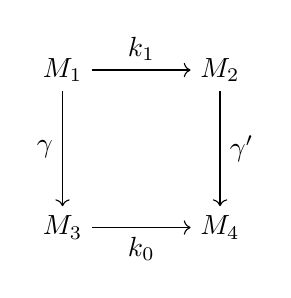
\begin{tikzpicture}[baseline=(current bounding box.center)]
        \node (M1) at (0,2) {$M_1$};
        \node (M2) at (2,2) {$M_2$};
        \node (M3) at (0,0) {$M_3$};
        \node (M4) at (2,0) {$M_4$};
        \draw[->] (M1) to node[above] {$k_1$} (M2);
        \draw[->] (M1) to node[left] {$\gamma$} (M3);
        \draw[->] (M2) to node[right] {$\gamma'$} (M4);
        \draw[->] (M3) to node[below] {$k_0$} (M4);
    \end{tikzpicture}
    \]
    whose image under $\mathrm{P}$ is a cartesian square in $\mathbf{A}$, if $\gamma$ and $\gamma'$ are cartesian and $k_0$ is cocartesian, then $k_1$ is cocartesian.
\end{itemize}
\end{definition}

\subsection{Characterization of Descent Data}

Assume henceforth that $\mathrm{P} : \mathbf{M} \to \mathbf{A}$ is a Chevalley functor. Let $a : A_1 \to A_0$ be an arrow in $\mathbf{A}$. Let $A_2$ be the fibred product $A_1 \times_{A_0} A_1$, with canonical projections $a_1, a_2 : A_2 \to A_1$. The property (C) defines, for every object $M_1 \in \mathbf{M}(A_1)$, a canonical bijection, natural in $M_1$,
\[
\operatorname{Hom}_{\mathbf{M}(A_2)}(a_1^*(M_1), a_2^*(M_1)) \to \operatorname{Hom}_{\mathbf{M}(A_1)}(T^a(M_1), M_1),
\]
denoted $\varphi \mapsto \mathrm{K}^a(\varphi)$.

\begin{lemma}
\label{lem:descent}
An arrow $\varphi : a_1^*(M_1) \to a_2^*(M_1)$ such that $\mathrm{P}(\varphi) = \mathrm{id}_{A_2}$ is a descent datum if and only if $\mathrm{K}^a(\varphi)$ is an algebra over the monad $\mathbf{T}^a$.
\end{lemma}

Let $\mathrm{D}(a)$ denote the category of descent data relative to $a$, and let
\[
\Psi^a : \mathbf{M}(A_0) \to \mathrm{D}(a), \quad \mathrm{U}^a : \mathrm{D}(a) \to \mathbf{M}(A_1)
\]
be the canonical functors.

\begin{theorem}
\label{thm:equivalence}
The correspondence $\varphi \mapsto \mathrm{K}^a(\varphi)$ induces an equivalence of categories $\mathrm{K}^a : \mathrm{D}(a) \to \mathbf{M}^a$, making the following diagram commute:
\[
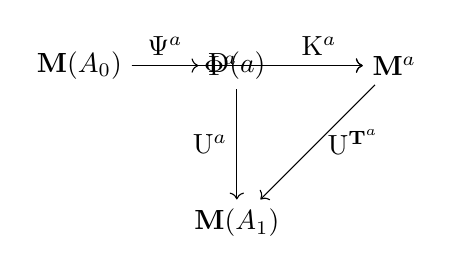
\begin{tikzpicture}
    \node (M0) at (0,2) {$\mathbf{M}(A_0)$};
    \node (Da) at (2,2) {$\mathrm{D}(a)$};
    \node (Ma) at (4,2) {$\mathbf{M}^a$};
    \node (M1) at (2,0) {$\mathbf{M}(A_1)$};
    \draw[->] (M0) to node[above] {$\Psi^a$} (Da);
    \draw[->] (Da) to node[above] {$\mathrm{K}^a$} (Ma);
    \draw[->] (M0) to node[left] {$\Phi^a$} (Ma);
    \draw[->] (Da) to node[left] {$\mathrm{U}^a$} (M1);
    \draw[->] (Ma) to node[right] {$\mathrm{U}^{\mathbf{T}^a}$} (M1);
\end{tikzpicture}
\]
\end{theorem}

\begin{proposition}
\label{prop:universal}
The correspondence $\varphi \mapsto \mathrm{K}^a(\varphi)$ is universal. Precisely, for an arrow $b_0 : A_0' \to A_0$ in $\mathbf{A}$, consider the change-of-base diagram in $\mathbf{A}$:
\[
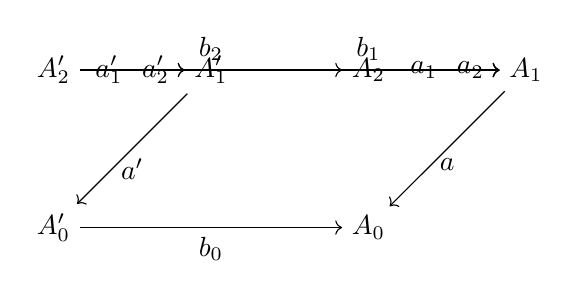
\begin{tikzpicture}
    \node (A2') at (0,2) {$A_2'$};
    \node (A1') at (2,2) {$A_1'$};
    \node (A0') at (0,0) {$A_0'$};
    \node (A2) at (4,2) {$A_2$};
    \node (A1) at (6,2) {$A_1$};
    \node (A0) at (4,0) {$A_0$};
    \draw[->] (A2') to node[above] {$b_2$} (A2);
    \draw[->] (A1') to node[above] {$b_1$} (A1);
    \draw[->] (A0') to node[below] {$b_0$} (A0);
    \draw[->] (A2') to node[left] {$a_1'$} (A1');
    \draw[->] (A2) to node[left] {$a_1$} (A1);
    \draw[->] (A2') to node[right] {$a_2'$} (A1');
    \draw[->] (A2) to node[right] {$a_2$} (A1);
    \draw[->] (A1') to node[below] {$a'$} (A0');
    \draw[->] (A1) to node[below] {$a$} (A0);
\end{tikzpicture}
\]
For $M_1 \in \mathbf{M}(A_1)$ and $\varphi : a_1^*(M_1) \to a_2^*(M_1)$ in $\mathbf{M}(A_2)$,
\[
\mathrm{K}^{a'}(b_2^*(\varphi)) = b_1^*(\mathrm{K}^a(\varphi)).
\]
\end{proposition}

In particular, taking $A_0' = A_1$ and $b_0 = a$, if $\varphi$ is a descent datum, then $b_2^*(\varphi)$ is an effective descent datum. The converse holds, yielding:

\begin{corollary}
\label{cor:effective-descent}
An arrow $\varphi : a_1^*(M_1) \to a_2^*(M_1) \in \mathbf{M}(A_2)$ is a descent datum if and only if its inverse image $b_2^*(\varphi)$ under the canonical change of base $b_0 = a : A_0' = A_1 \to A_0$ is an effective descent datum.
\end{corollary}

This eliminates the need for the ``cocycle condition'' in subsequent arguments.

\section{First Applications}

Using Theorem \ref{thm:equivalence}, Beck's criterion \cite{Linton1969} provides necessary and sufficient conditions for $\Psi^a$ to be faithful, fully faithful, or an equivalence of categories, in terms of commutation and reflection of certain cokernels by $a^*$.

\begin{proposition}
\label{prop:adj-left}
If cokernels of pairs of arrows exist in $\mathbf{M}(A_0)$, then $\Psi^a$ has a left adjoint.
\end{proposition}

\begin{proposition}
\label{prop:faithful}
The functor $\Psi^a$ is faithful if and only if $a^*$ is faithful.
\end{proposition}

\begin{proposition}
\label{prop:fully-faithful}
If $a^*$ reflects cokernels, then $\Psi^a$ is fully faithful. In particular, if all fibres of $\mathbf{M}$ are abelian, then
\[
\Psi^a \text{ faithful} \iff \Psi^a \text{ fully faithful} \iff a^* \text{ faithful}.
\]
\end{proposition}

\begin{definition}
\label{def:faithfully-flat}
An arrow $a : A_1 \to A_0$ is \emph{faithfully flat} if $a^*$ commutes with cokernels and reflects isomorphisms.
\end{definition}

\begin{proposition}
\label{prop:equivalence}
If $a : A_1 \to A_0$ is faithfully flat and cokernels exist in $\mathbf{M}(A_0)$, then $\Psi^a$ is an equivalence of categories.
\end{proposition}

\section{First Examples of Chevalley Functors}

\begin{enumerate}
    \item If $\mathbf{A}$ is the dual of the category of commutative rings and $\mathbf{M}$ is the dual of the category of modules over varying commutative rings, the obvious functor $\mathrm{P} : \mathbf{M} \to \mathbf{A}$ is Chevalley.
    \item If $\mathbf{A}$ is a category with fibred products and $\mathbf{M} = \mathbf{Fl}(\mathbf{A})$ is the category of arrows in $\mathbf{A}$, the ``target'' functor $\mathrm{P} : \mathbf{M} \to \mathbf{A}$ is Chevalley.
    \item If $\mathrm{P} : \mathbf{M} \to \mathbf{A}$ and $\mathrm{Q} : \mathbf{N} \to \mathbf{M}$ are Chevalley, their composite $\mathrm{P} \circ \mathrm{Q}$ is Chevalley.
    \item If $\mathrm{P} : \mathbf{M} \to \mathbf{A}$ is Chevalley and $\mathbf{I}$ is any category, the functor $\mathrm{P}^{\mathbf{I}} : \mathbf{M}^{\mathbf{I}} \to \mathbf{A}^{\mathbf{I}}$ is Chevalley.
    \item In a cartesian diagram of categories
    \[
    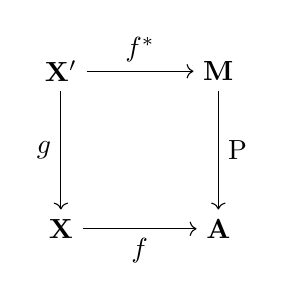
\begin{tikzpicture}
        \node (X') at (0,2) {$\mathbf{X}'$};
        \node (M) at (2,2) {$\mathbf{M}$};
        \node (X) at (0,0) {$\mathbf{X}$};
        \node (A) at (2,0) {$\mathbf{A}$};
        \draw[->] (X') to node[above] {$f^*$} (M);
        \draw[->] (X') to node[left] {$g$} (X);
        \draw[->] (M) to node[right] {$\mathrm{P}$} (A);
        \draw[->] (X) to node[below] {$f$} (A);
    \end{tikzpicture}
    \]
    if $\mathbf{X}$ has fibred products, $f$ preserves fibred products, and $\mathrm{P}$ is Chevalley, then $f^*(\mathrm{P})$ is Chevalley.
\end{enumerate}

In a future publication, we will provide further examples of Chevalley categories and more precise criteria for determining whether $\Psi^a$ is faithful, fully faithful, or an equivalence when the fibres of $\mathbf{M}$ are algebraic categories (e.g., categories of modules).

\begin{thebibliography}{9}
\bibitem{Grothendieck1959} A. Grothendieck, Cat\'egories fibr\'ees et descente, \emph{S\'eminaire Bourbaki}, 1959.
\bibitem{Linton1969} F. E. J. Linton, Applied functorial semantics II, \emph{Springer Lecture Notes in Mathematics}, No. 80, 1969.
\bibitem{Chevalley1964} C. Chevalley, S\'eminaire sur la descente, 1964--1965 (unpublished).
\end{thebibliography}

\end{document}
